Android is an open source mobile \gls{os} launched in 2007 and today mainly maintained and developed by Google.
It is based on the Linux kernel and mainly targets touch screen devices such as mobile devices or wearables.
The system is designed to run efficiently on battery powered devices with limited hardware and computational capacity.
Android's main hardware platform is the ARM architecture, known for their low power consumption, are mainly used in this scenario.
The following will give an overview over the architecture of Android and a deeper insight in the runtime system powering Android.
The architecture of the software stack of Android can be seen in figure~\ref{fig:androidArchitecture}.
\newline

\begin{figure}[h]
    \centering
    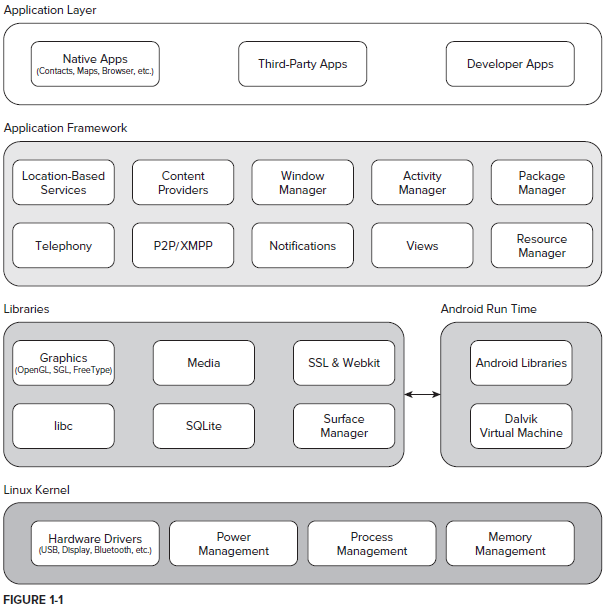
\includegraphics[width=0.8\textwidth]{data/stack.png}
    \caption{Android's architecture \cite{androidStack}}
    \label{fig:androidArchitecture}
\end{figure}

The basis of the system is its kernel.
It is responsible for power and memory management and controls the device drivers.
\newline
The layer above the kernel contains the Android Runtime, which will be explained in detail in section~\ref{subsection:android-art}, as well as the native libraries of the system.
Usually Android libraries are written in Java except the ones which are resource and time critical.
They are written in C or C++ in order to boost performance and allow low level interaction between applications and the kernel by using the \gls{jni}.
Examples for native libraries are OpenGL, multimedia playback or the SQLite database.
\newline
On top of the libraries and the runtime lies the application framework.
This layer provides generic functionality as notification support to applications over Android's \gls{api}.
\newline
The top layer enables the installation and execution of applications.
\newline
Using these layers and abstraction enables Android to be run on a wide range of devices as well allows software to execute standard Unix commands using the kernel.
